\section{Spezifische Anforderungen}
\subsection{Funktionale Anforderungen}
\subsubsection{DFD1 Simulation}
\begin{figure}[H]
	\centering
  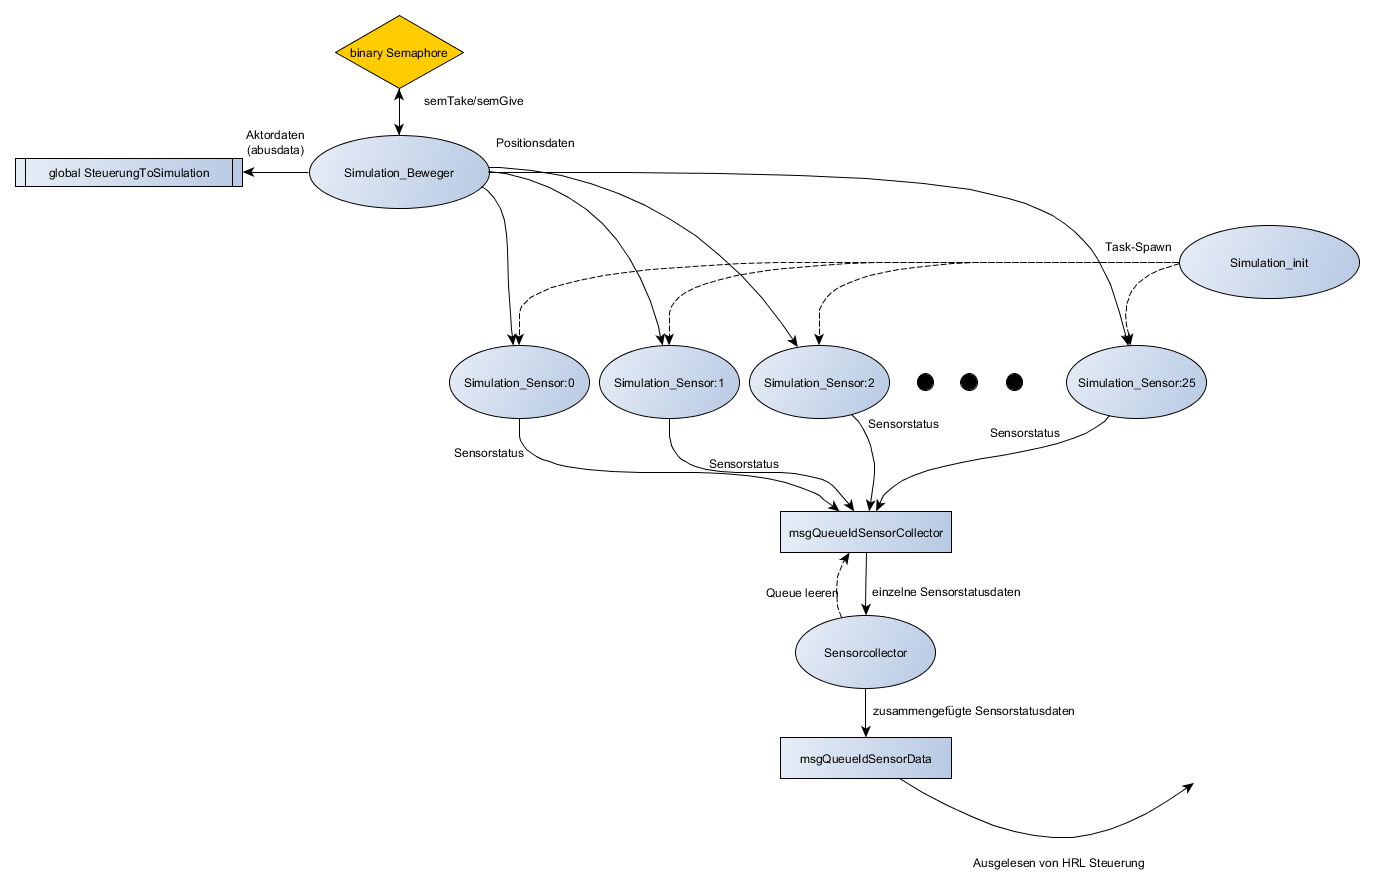
\includegraphics[width=\textwidth]{DFD/dfd1_simulation1_1.png}
	\caption{DFD1 Simulation}
	\label{fig1}
\end{figure}
\paragraph{Sensorcollector}
Der \textbf{Sensorcollector} sammelt aus der \textbf{MessageQueue} die Einträge aller Sensoren. Wenn ein Sensor ausfällt bleibt der Wert des Sensors auf 1.